\section{The Universal Base}
The aim for this project was to create an all-purpose, powerful chassis that is lighter, simpler, and more maintainable than previous designs; Doing this would allow us to very quickly switch from competition to competition without re-building the entire robot from scratch, as well fix the robot easily.

\begin{figure}[h]
    \centering
    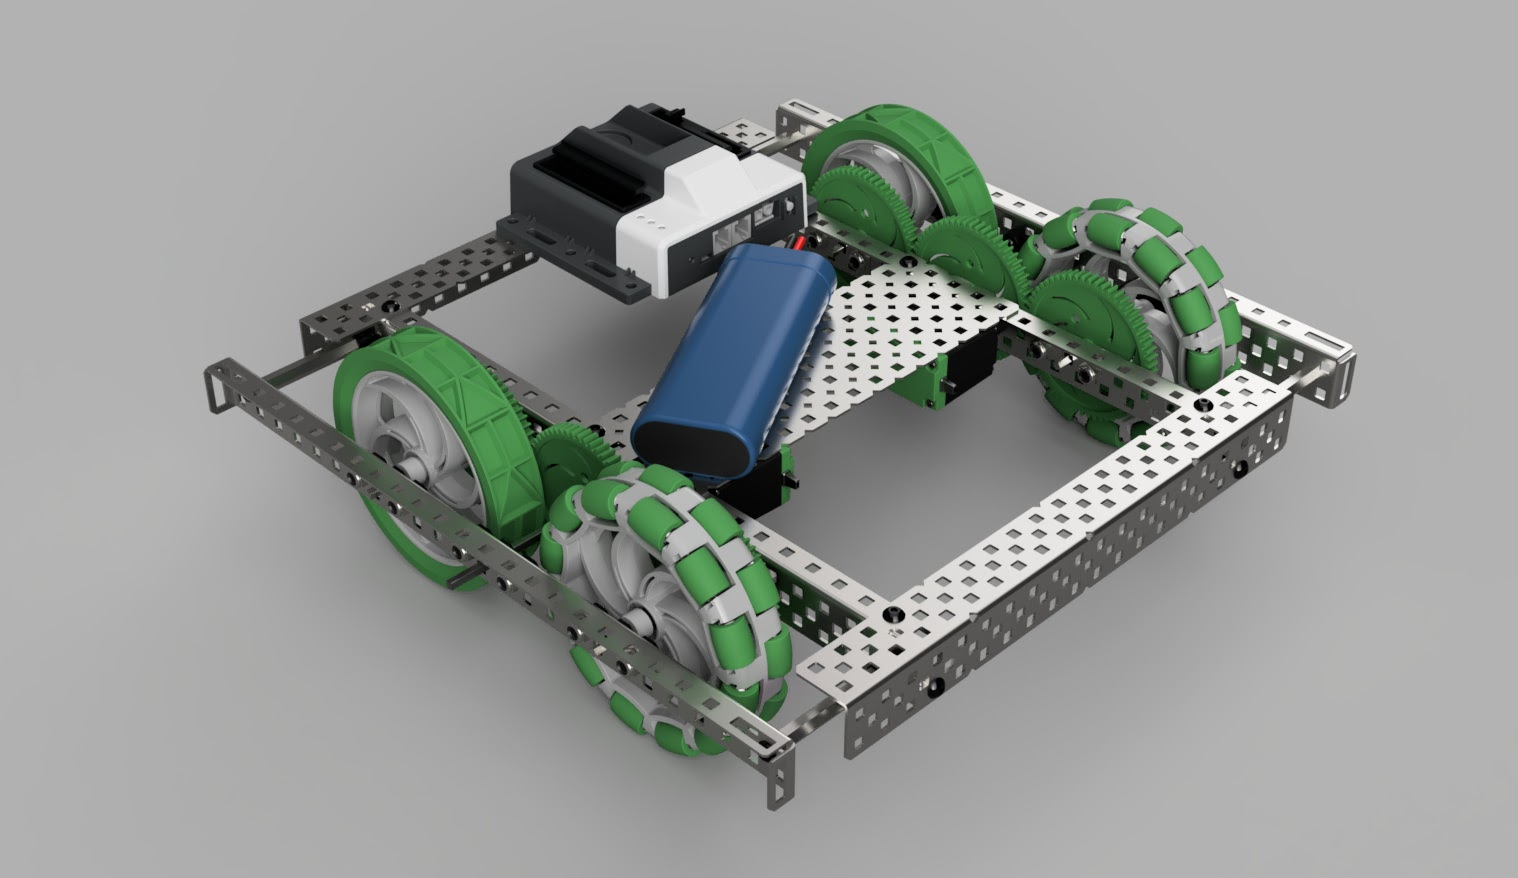
\includegraphics[width=\textwidth,height=4cm,keepaspectratio=true]{CADChassis}
    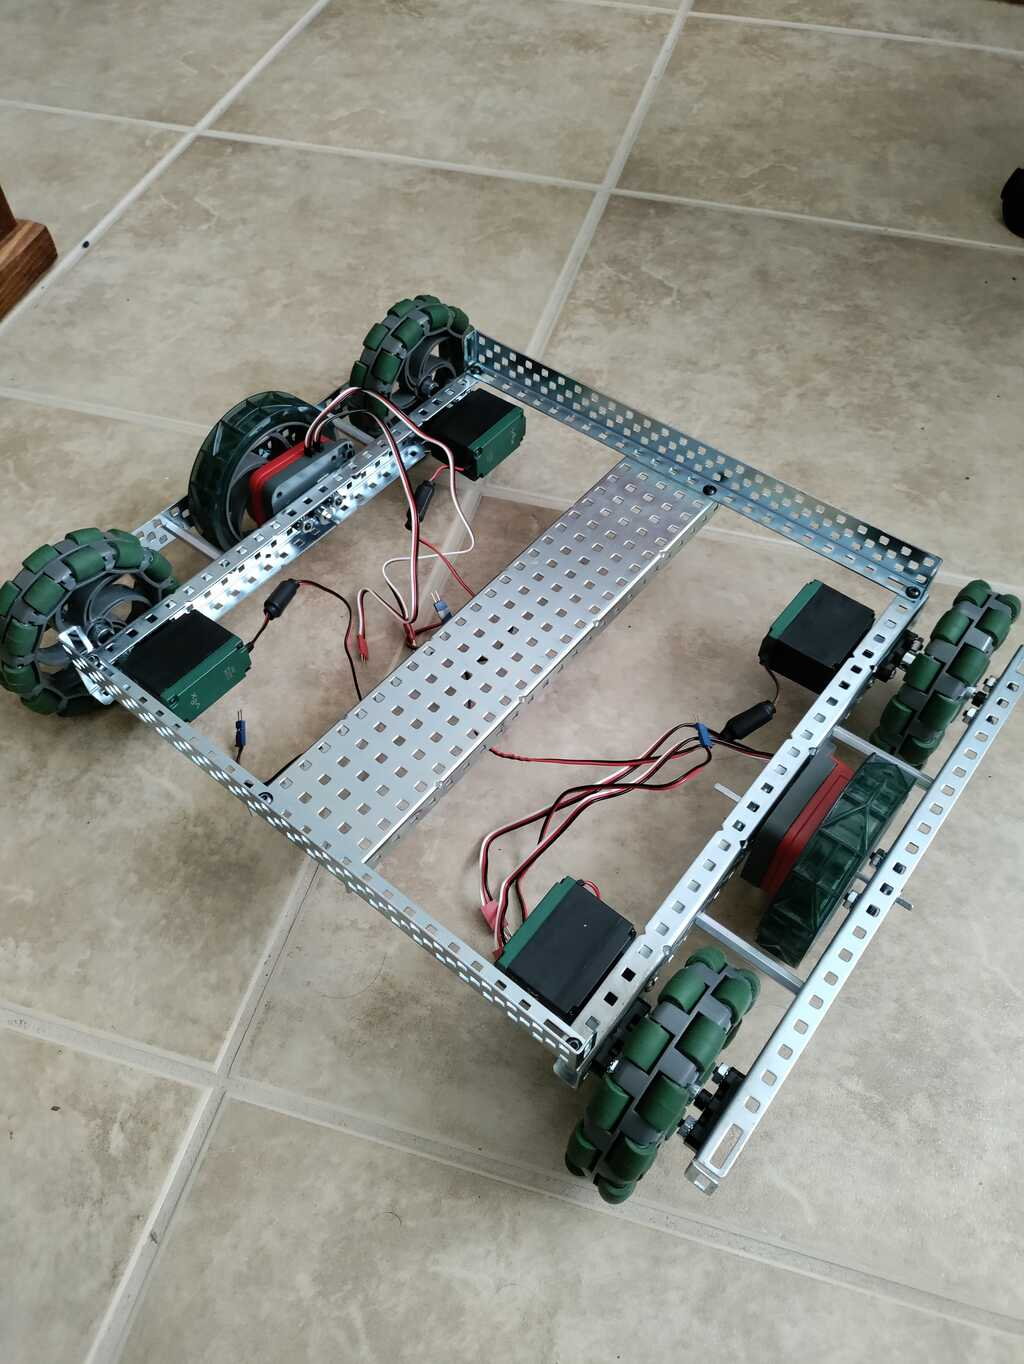
\includegraphics[width=\textwidth,height=4cm,keepaspectratio=true]{V1}
    \caption{
        (Left) An old 3D model showing a potential chassis supported by standoffs. (Right) Prototype of the proposed design using the same principle.
    }
\end{figure}

The idea was to switch over to a 4-motor chassis that had its axes supported on both sides via standoffs; Standoffs were chosen due to requiring less metal, having an easier location to tighten, and allowing for a more flexible chassis width, as shown in the CAD. A 4-motor design was chosen due to requiring less moving parts as well as having more torque. However, in addition to 4 individually powered wheels, two unpowered wheels were going to be added in the axis of rotation, or the center, so as to give attached encoders very good accuracy.

\begin{figure}[h]
    \centering
    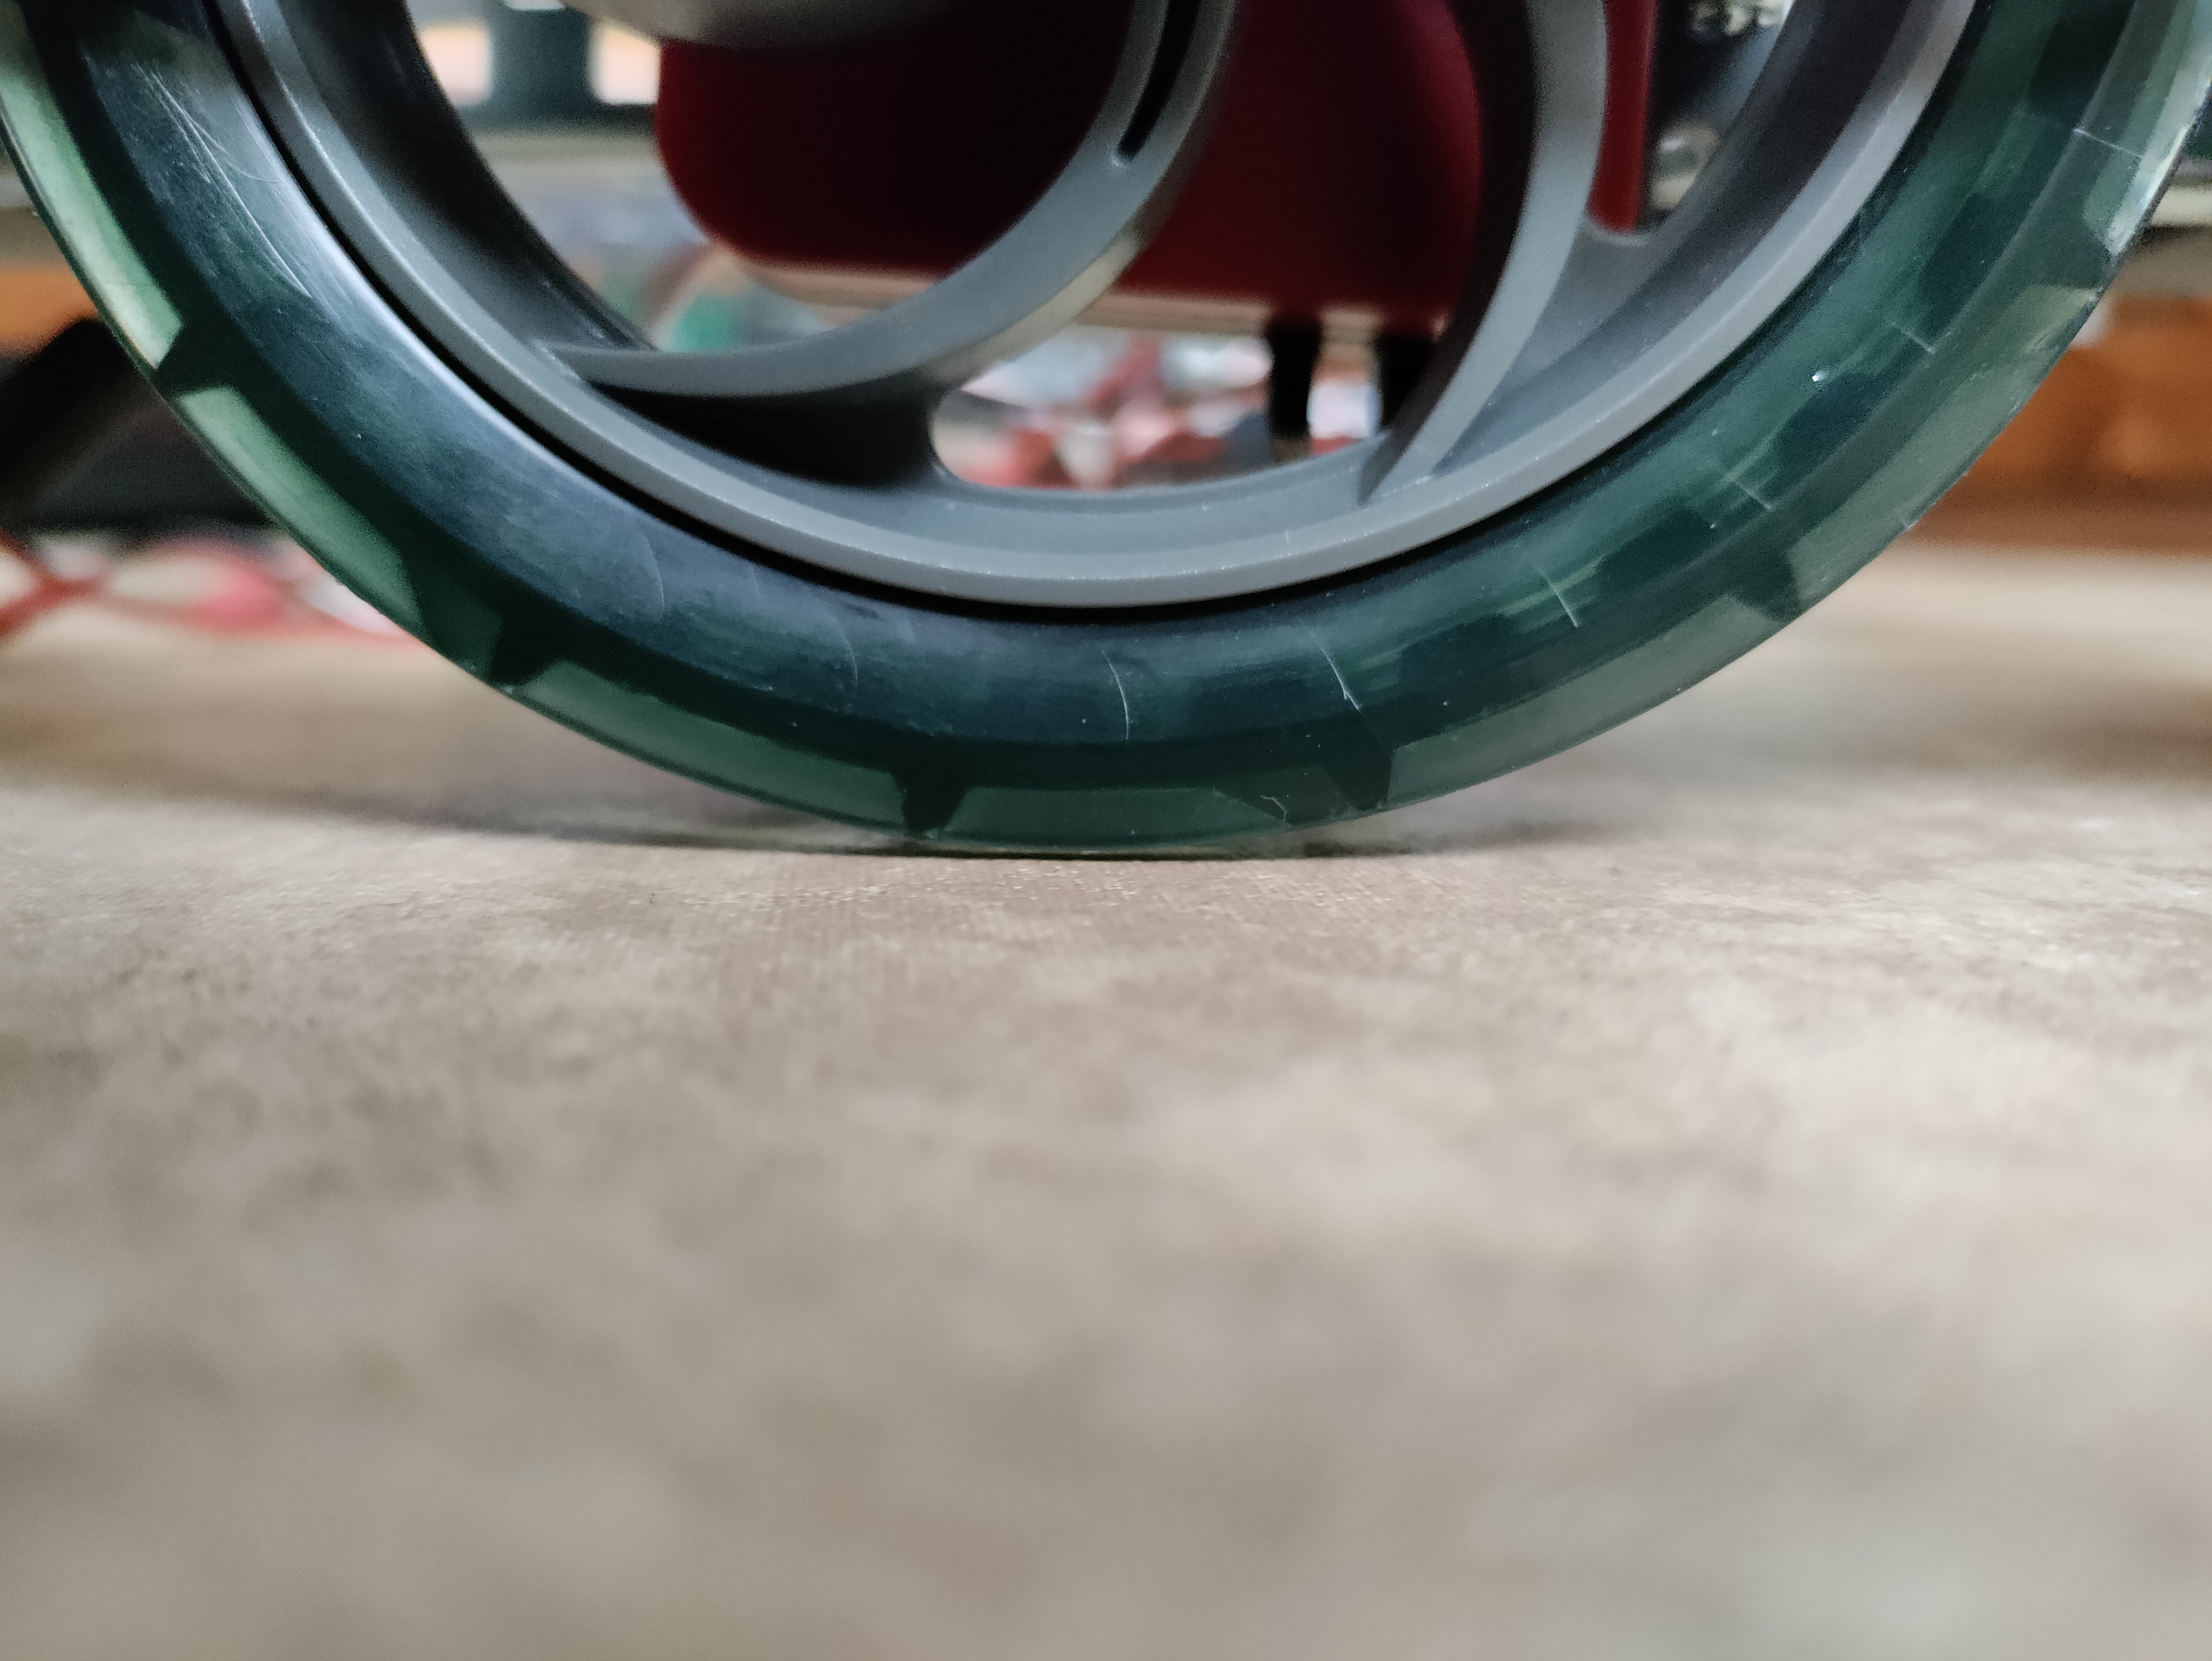
\includegraphics[width=\textwidth,height=3cm,keepaspectratio=true]{OGWheels}
    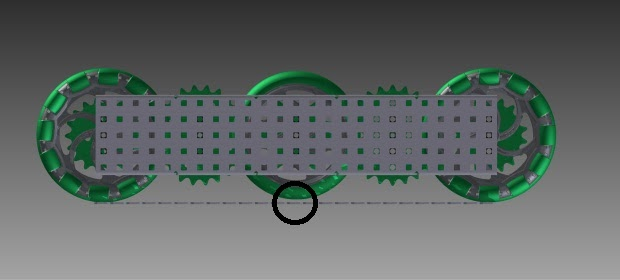
\includegraphics[width=\textwidth,height=3cm,keepaspectratio=true]{CADWheels}
    \caption{
        (Left) The prototype's wheel being literal microns off a tiled floor. (Right) A 3D model showing that the difference in size is caused by the wheels themselves, not any external factor.
    }
\end{figure}

Upon building the chassis, it was apparent that the unpowered traction wheels were not touching the ground. On closer inspection, I found out that holonomic wheels were a literal millimeter bigger in diameter, as shown in the CAD. While this may not be a problem in carpet or foam environments where the floor has some give, my hard tile floor made it near impossible for the two traction wheels to gain any traction.

\begin{figure}[h]
    \centering
    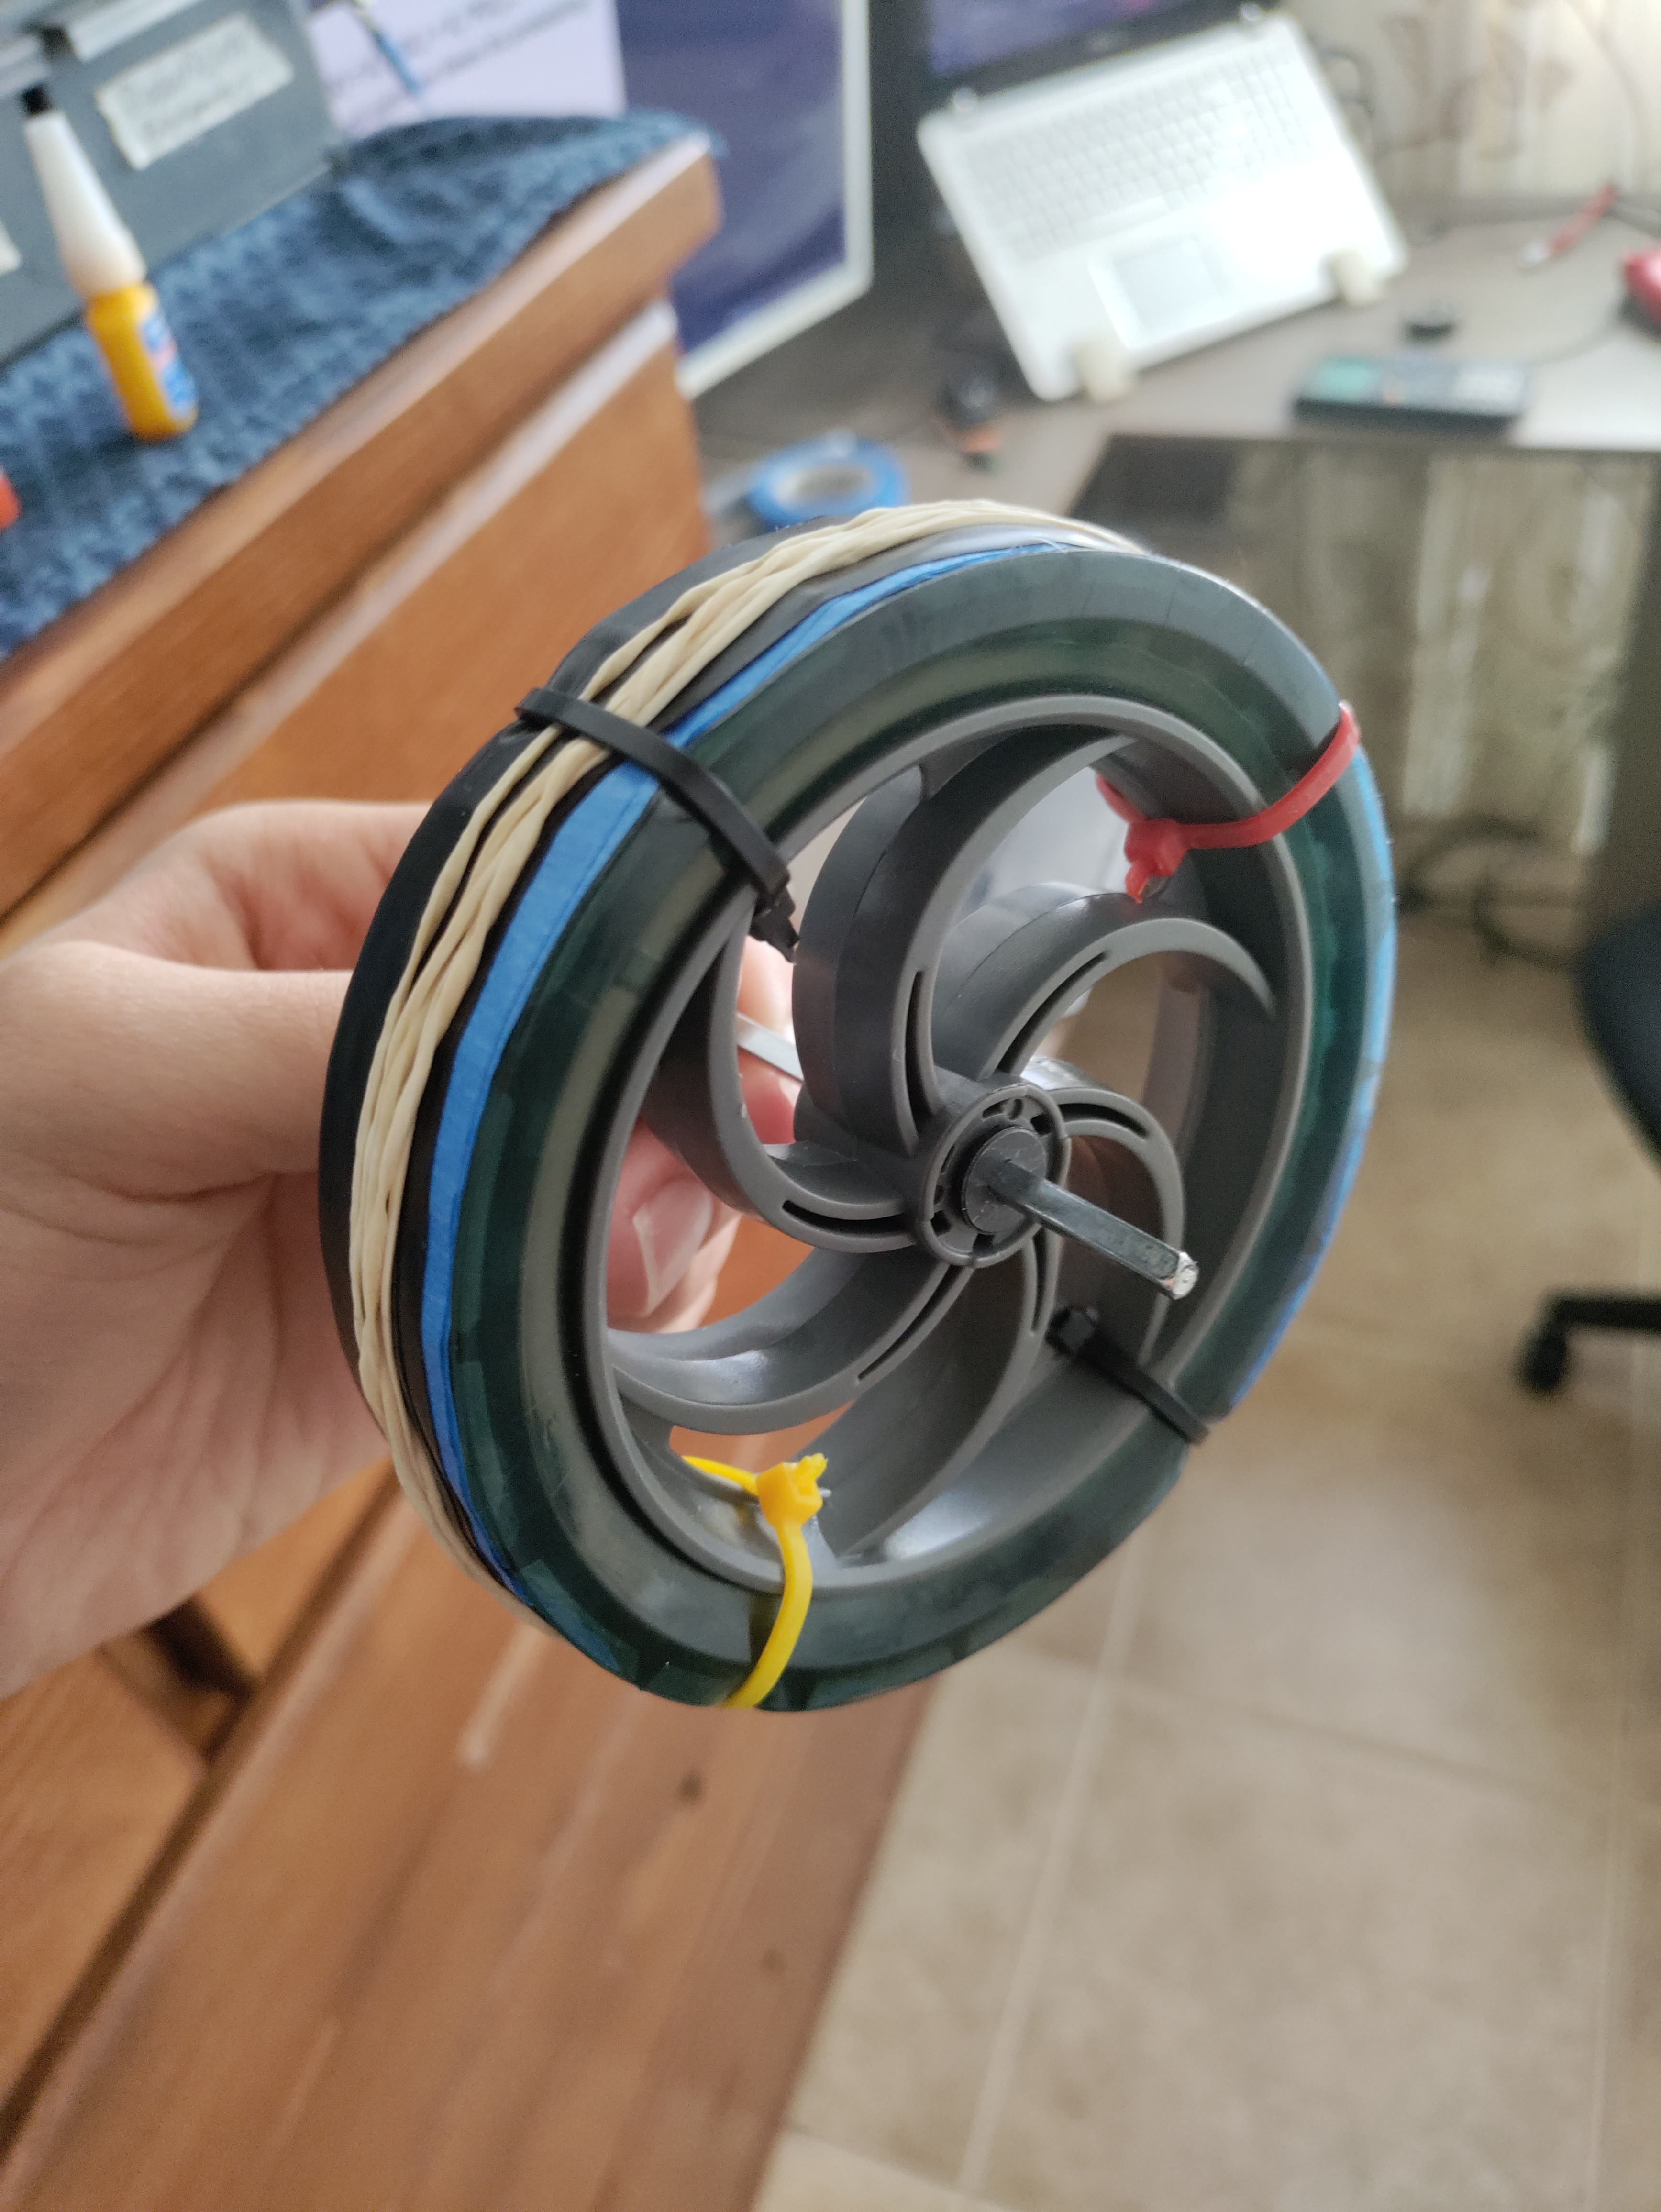
\includegraphics[width=\textwidth,height=6cm,keepaspectratio=true]{SuperWheel}
    \caption{
        A super wheel.
    }
\end{figure}

So I made, in lack of a better name, "super wheels". These wheels have 4 layers of Scotch Painter's tape, 2 layers of electrical tape, a few rubber bands, and 4 zipties 90 degrees apart from each other. The scotch tape is filler, the electrical tape and rubber bands are for traction, and the zip ties are so the rubber bands don't fall off. When these wheels are attached to the chassis, they are able to touch the floor with even more grip than regular traction wheels. As they are placed on the axis of rotation, the extra traction does not cause any turning scrub \cite{TurningScrub} that would otherwise make turning inefficient.

With the prototype showing very promising results, I rebuilt the robot in a way where it's very maintainable. Mainly, I flipped the side metal bars so that the shaft collars holding the wheels together are exposed, so that you can easily remove and attach the wheels in case anything goes wrong. I also made extra sure all screws holding the robot together were screwed outside to in, making it very easy to tighten nearly all parts of the robot without awkwardly tightening it from the inside.

All in all, the maximum size of the robot is 18" x 15.5" if it were built with the same parts; 17" x 15.5" if we are really cocky and take very special care building it. If for any reason the building constraints shrink, we can swap the X-axis and Y-axis bars with 15-hole C-channel, ditch the encoder wheels, and get the smallest possible size of 13" x 10".

\subsection{The Process}
The process of solving the tiny-gap issue.

\begin{figure}[h]
    \centering
    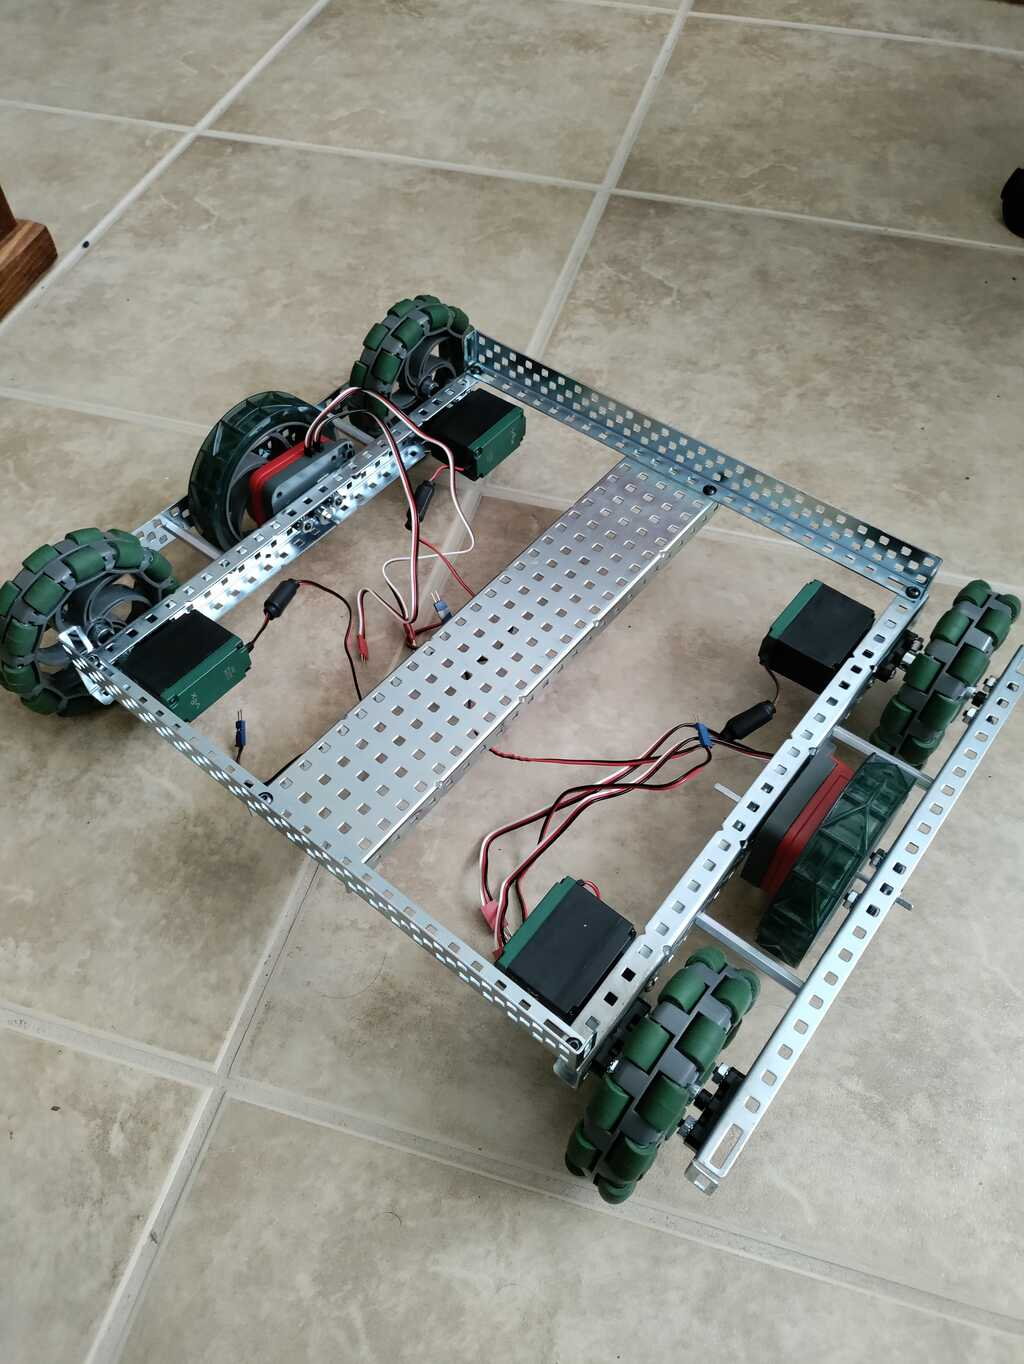
\includegraphics[width=\textwidth,height=5cm,keepaspectratio=true]{V1}
    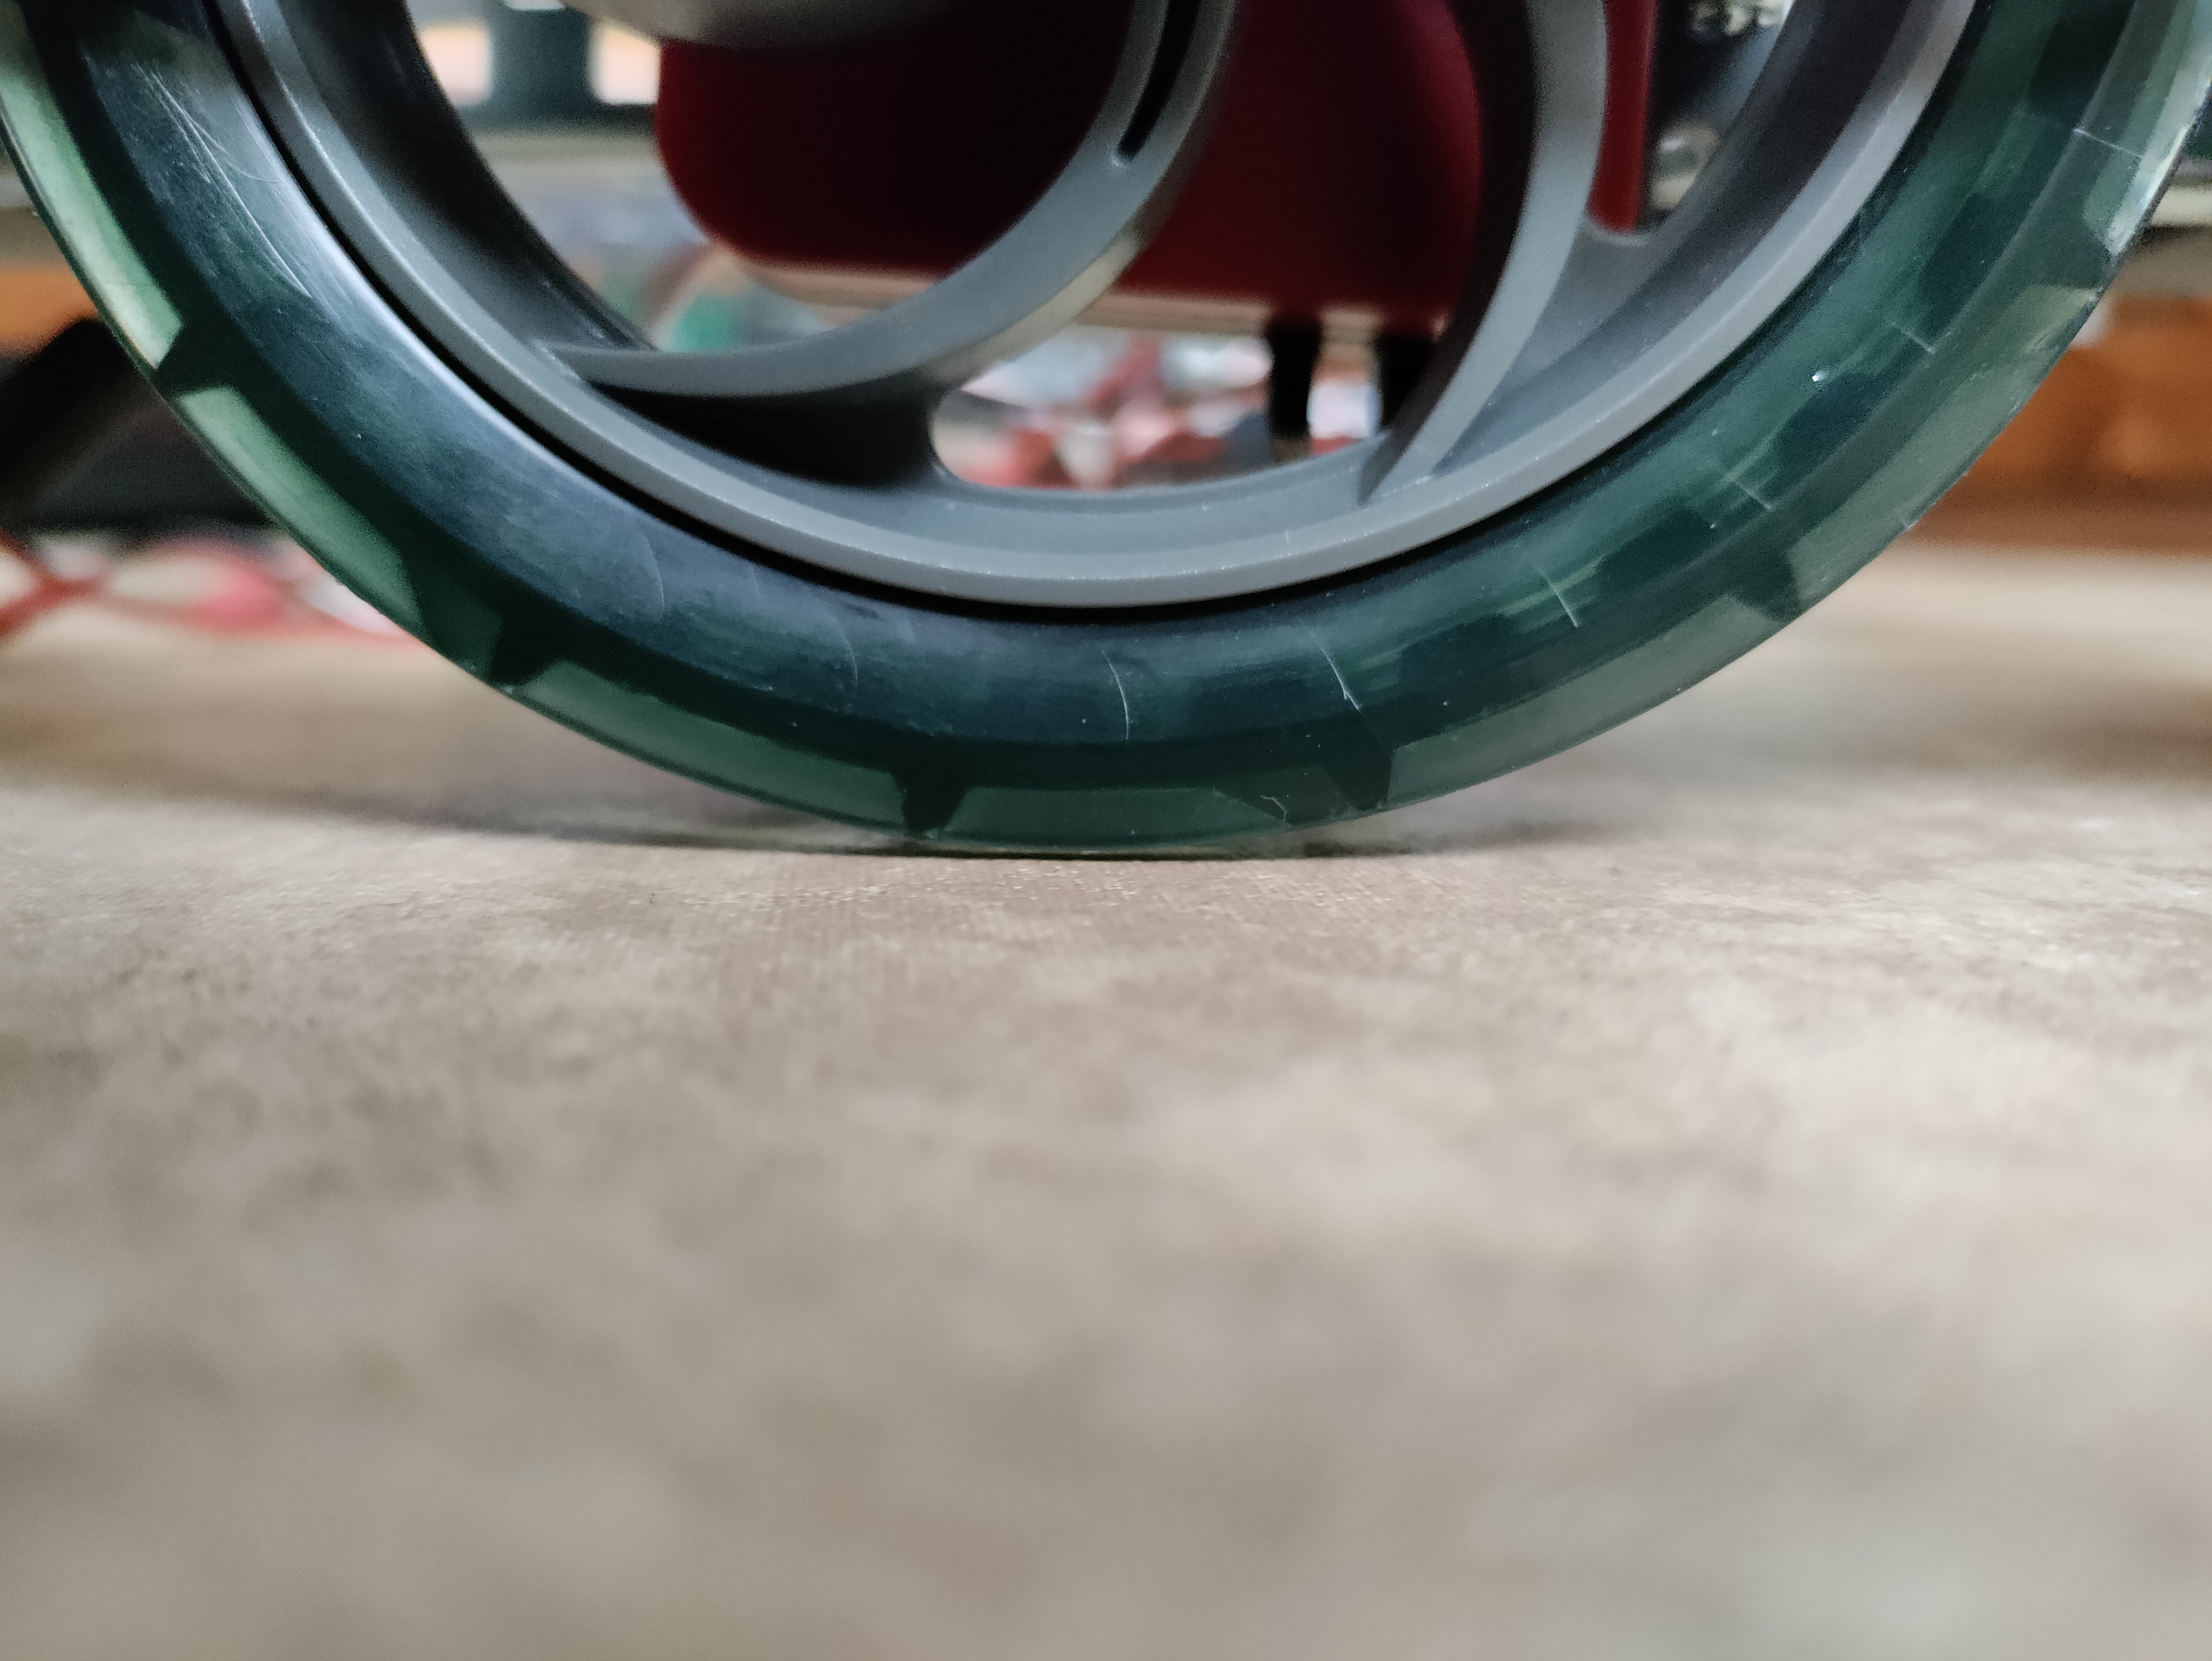
\includegraphics[width=\textwidth,height=5cm,keepaspectratio=true]{OGWheels}
    \caption{
        V1; Where the issue presented itself.
    }
\end{figure}

\begin{figure}[h]
    \centering
    \includegraphics[width=\textwidth,height=5cm,keepaspectratio=true]{V2Front}
    \includegraphics[width=\textwidth,height=5cm,keepaspectratio=true]{V2Side}
    \caption{
        V2; Added multiple layers of blue tape and a rubber band. The wheel made contact just fine, but it was slippery, lifted other wheels up, and jammed itself when the rubber band came loose. Hope was lost.
    }
\end{figure}

\begin{figure}[h]
    \centering
    \includegraphics[width=\textwidth,height=6cm,keepaspectratio=true]{V3}
    \caption{
        V3; Removed the wheels and called it a day (I was about to end it here).
    }
\end{figure}

\begin{figure}[h]
    \centering
    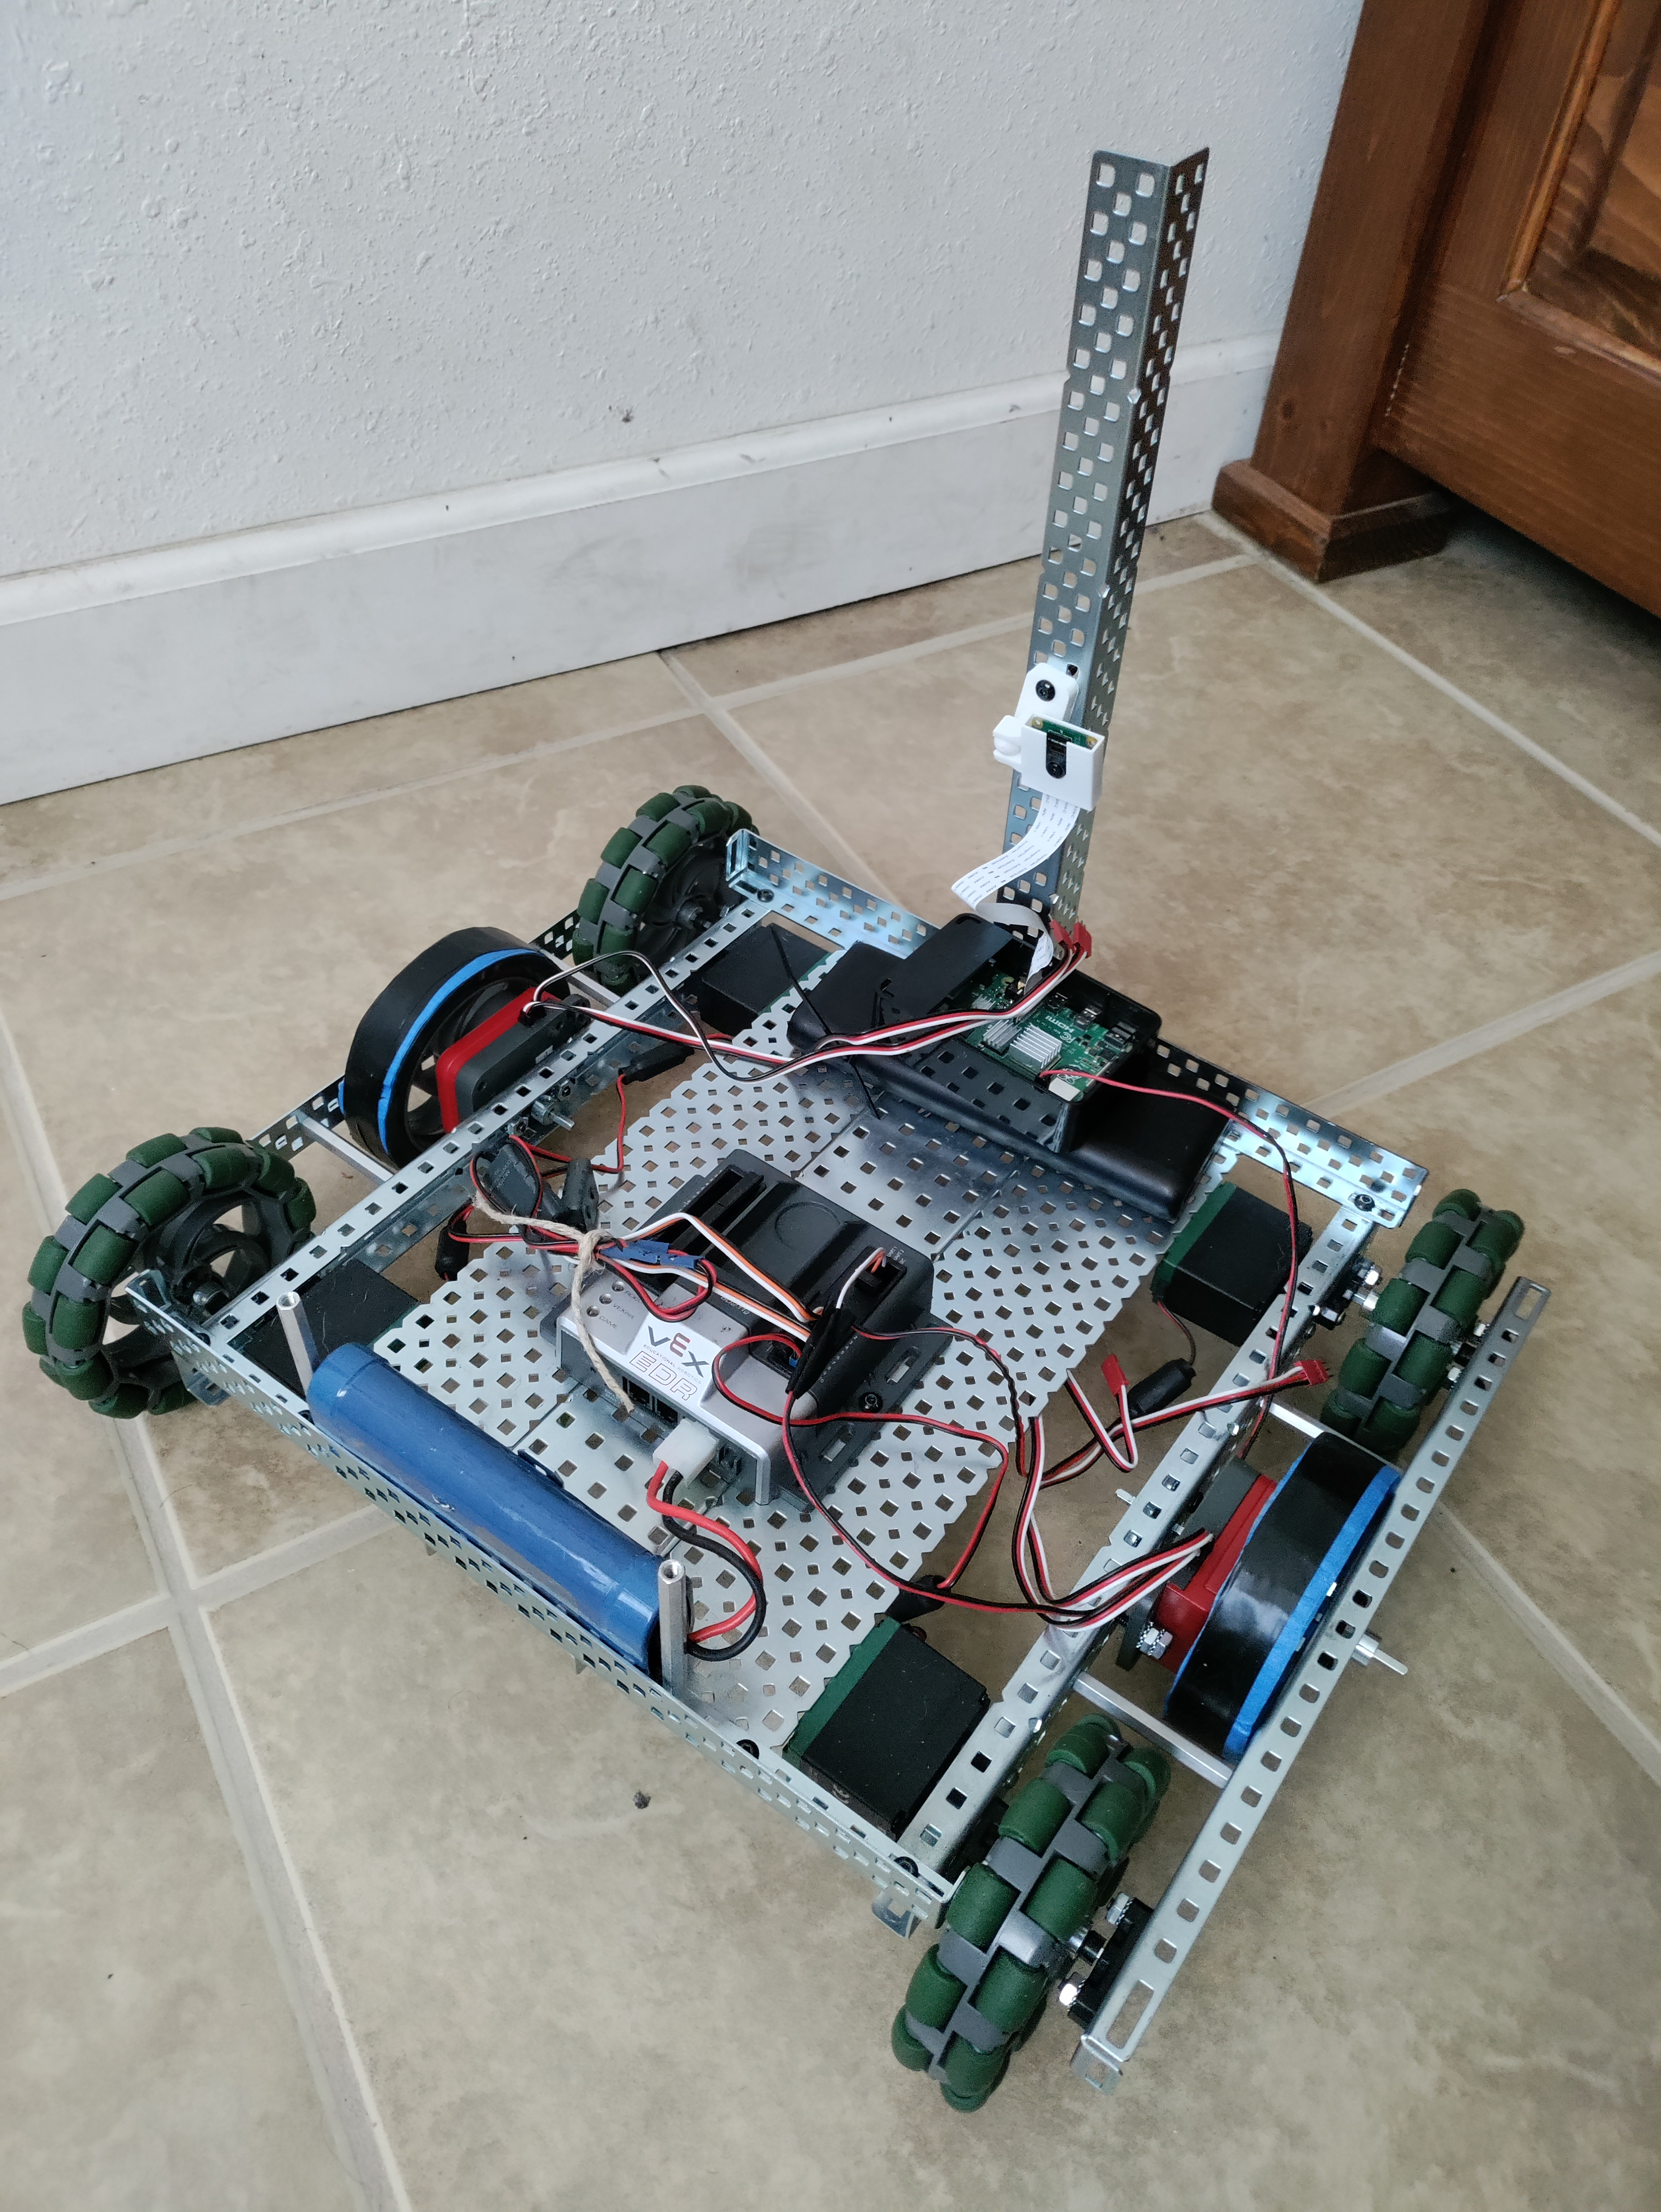
\includegraphics[width=\textwidth,height=6cm,keepaspectratio=true]{V4}
    \caption{
        V4; Got inspiration from electrical tape and slapped it on with blue tape as filler. Worked a lot better, though the traction caused it to sometimes slip on the valleys of the tile.
    }
\end{figure}

\begin{figure}[h]
    \centering
    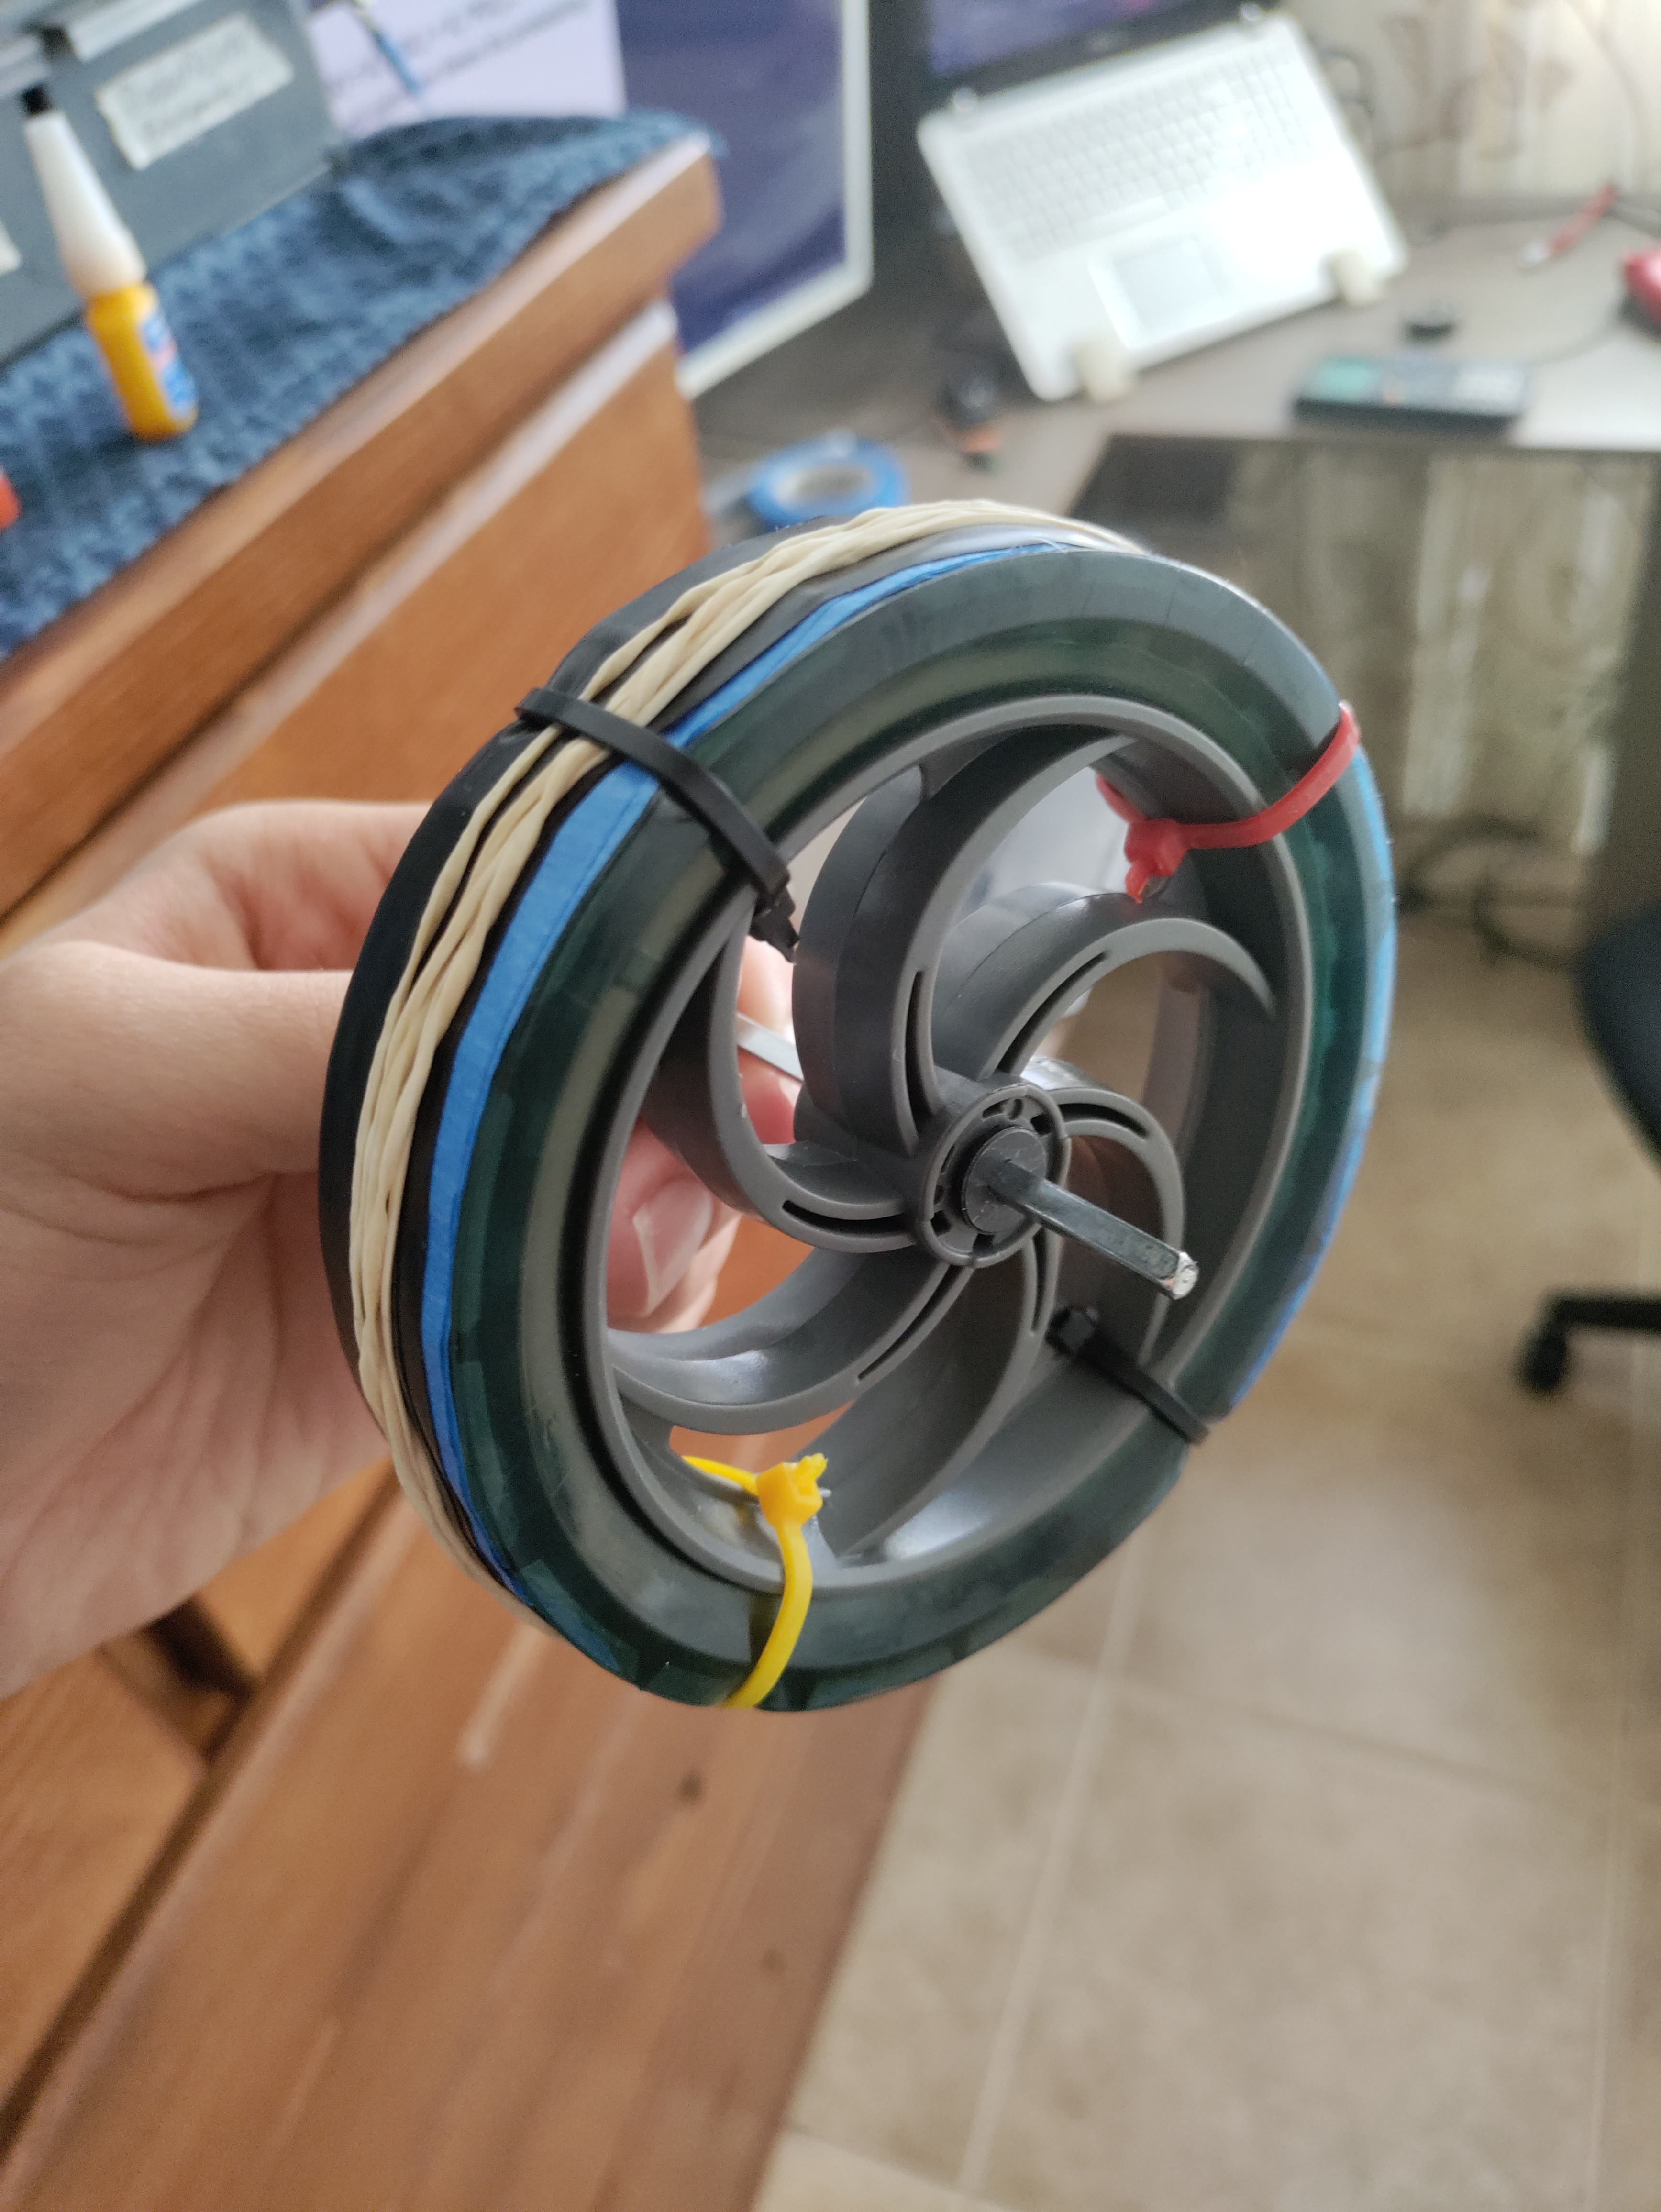
\includegraphics[width=\textwidth,height=4cm,keepaspectratio=true]{SuperWheel}
    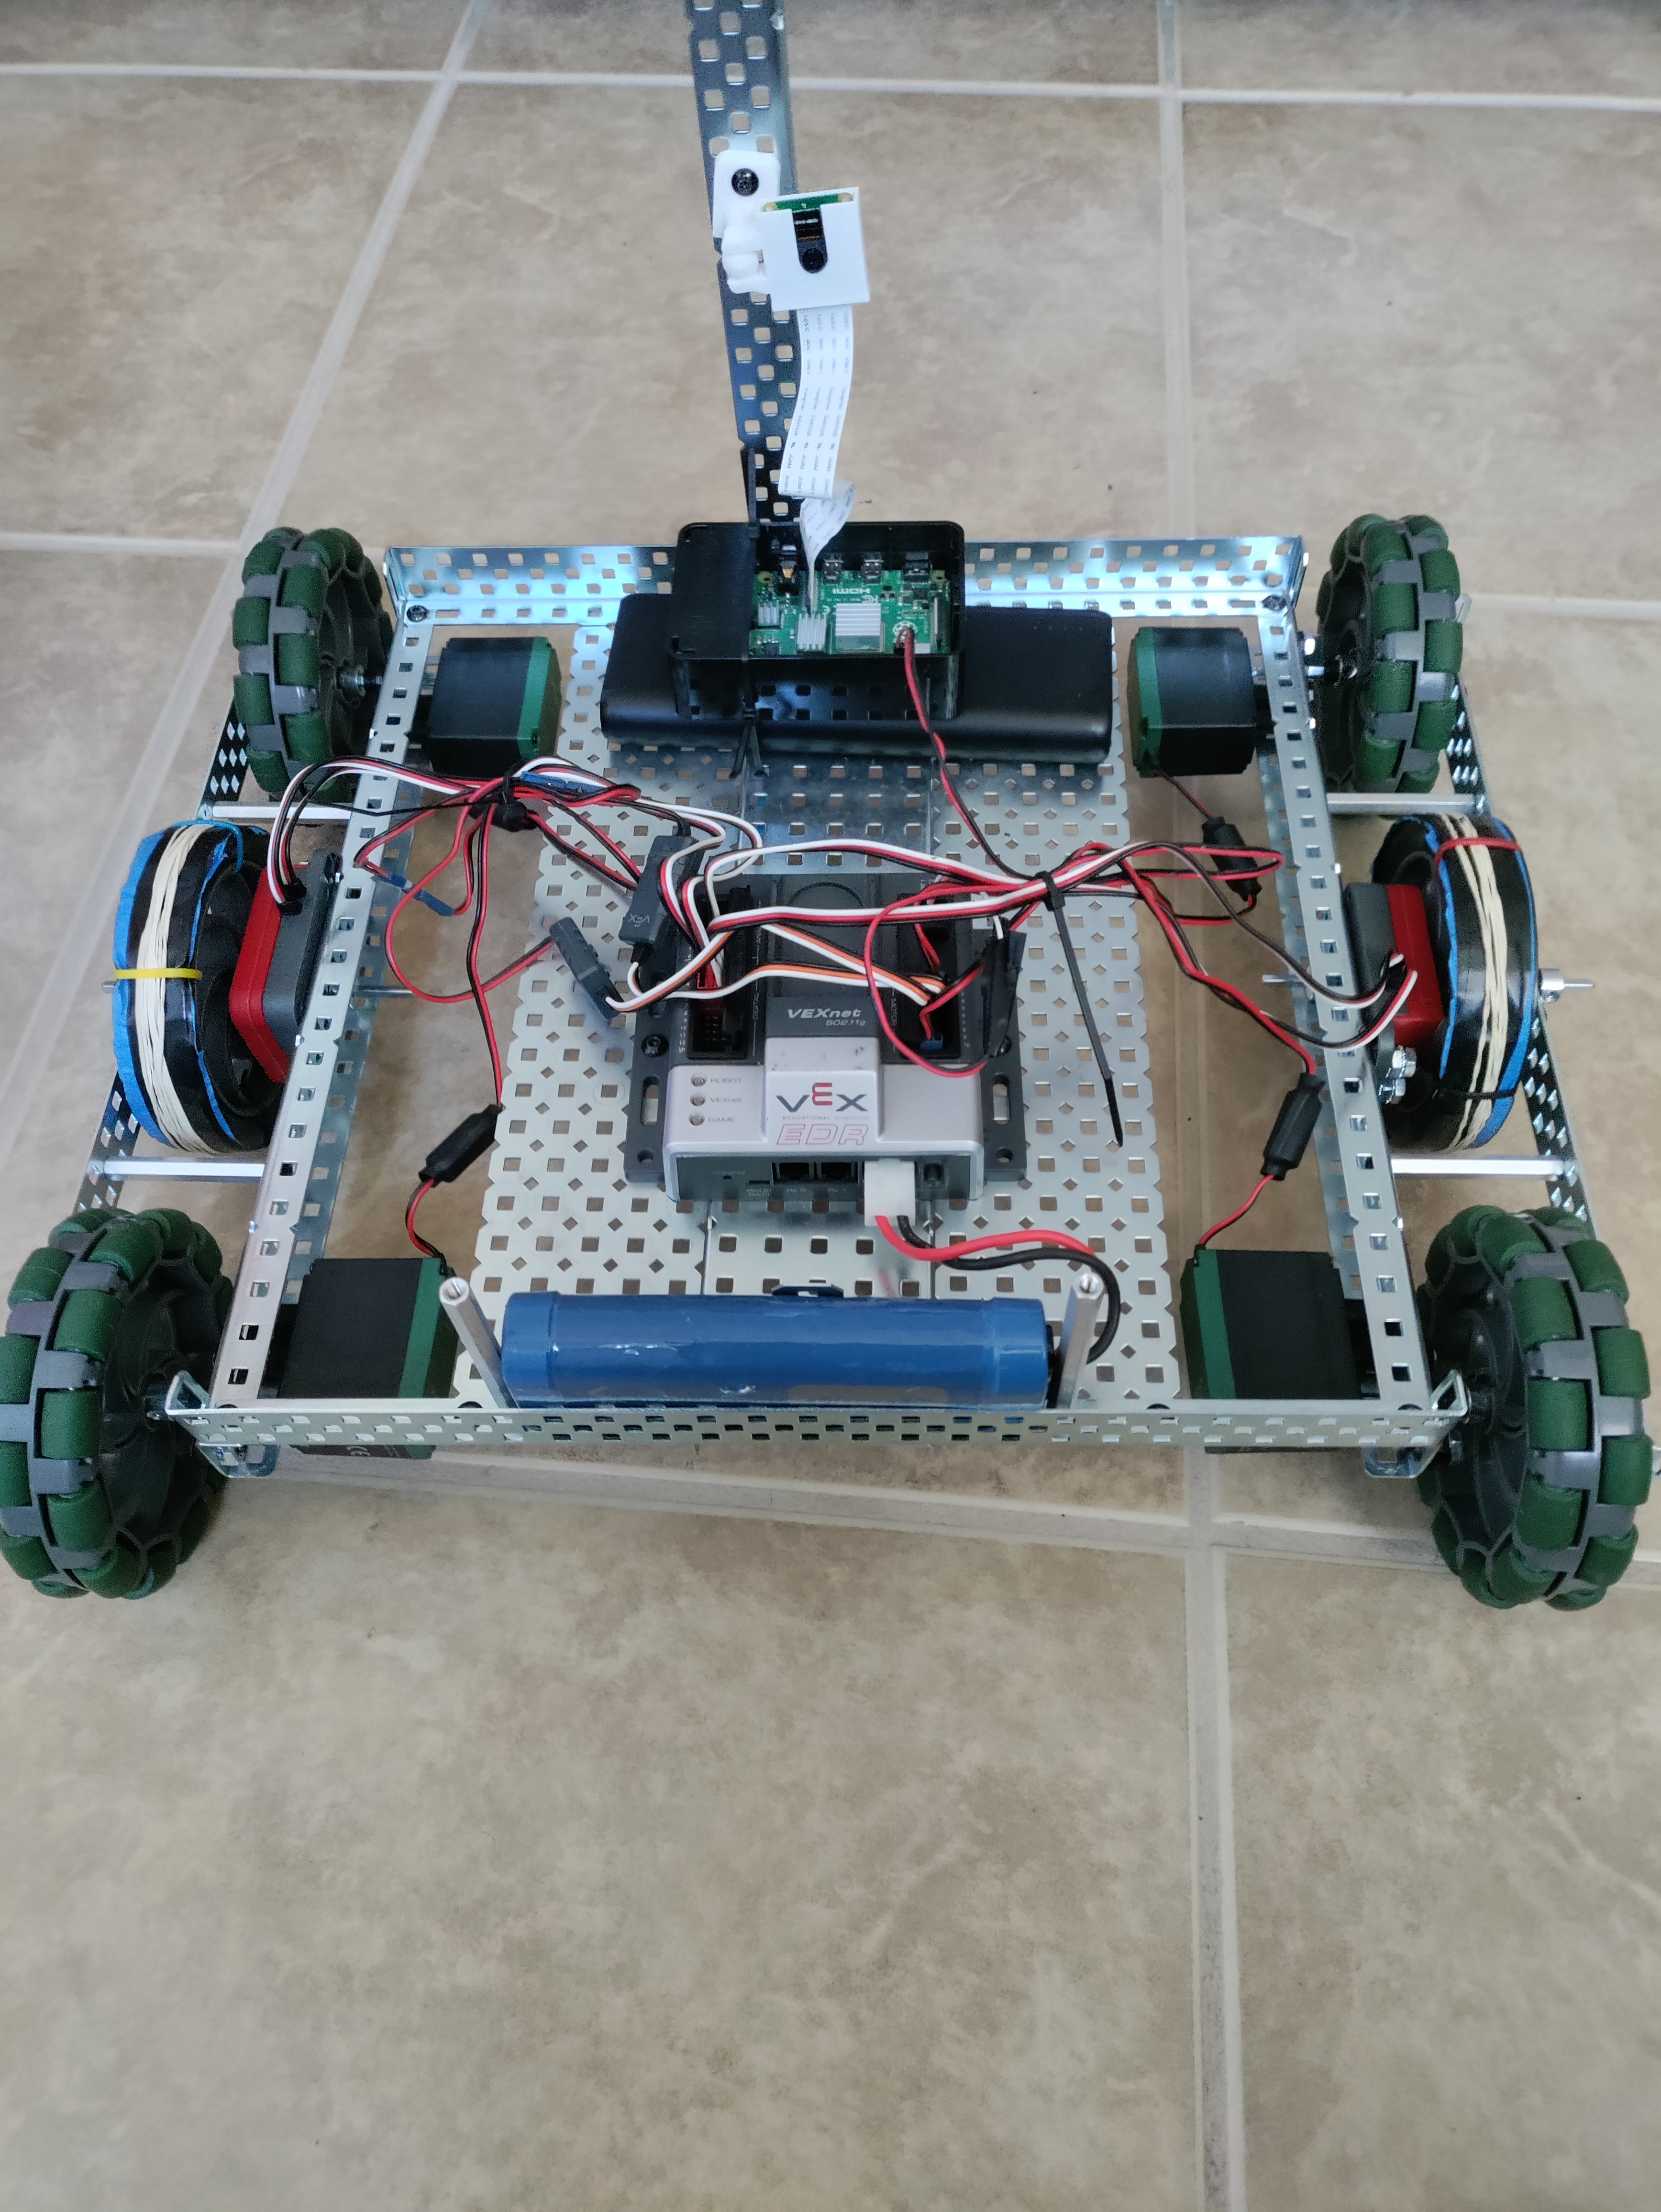
\includegraphics[width=\textwidth,height=4cm,keepaspectratio=true]{V5Front}
    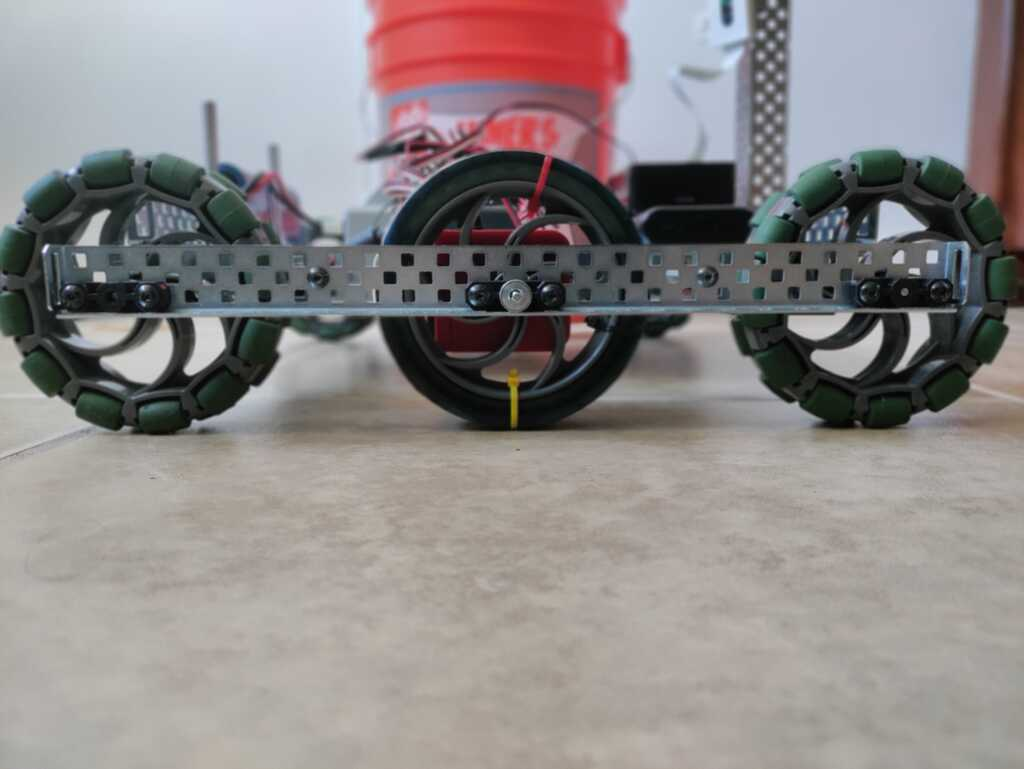
\includegraphics[width=\textwidth,height=4cm,keepaspectratio=true]{V5Side}
    \caption{
        V5 (Final); Rebuilt the robot with maintenance in mind and tried the super wheels. Works like a charm. I initially thought the zip ties would cause the robot to skip a lot, but it is not the case. As you can see, the axles are mounted at the very bottom of the metal; This is so that the encoder can properly be mounted on the axle, as well as to make the robot look a bit more fierce with height.
    }
\end{figure}


\begin{figure}[h]
    \centering
    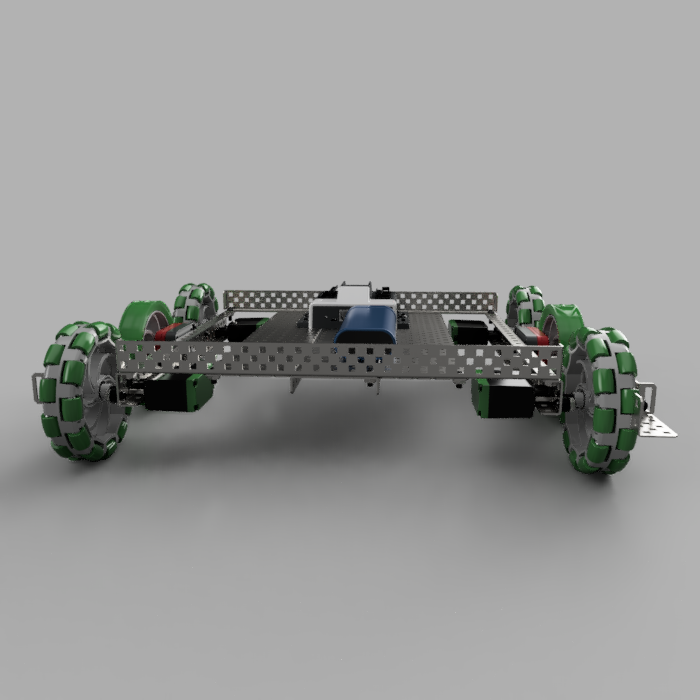
\includegraphics[width=\textwidth,height=7cm,keepaspectratio=true]{V5CAD}
    \caption{
        V5 (Final); The CAD in all its glory.
    }
\end{figure}
